\documentclass[8pt,aspectratio=169]{beamer}
\usetheme{Madrid}
\usepackage{graphicx}
\usepackage{booktabs}
\usepackage{adjustbox}
\usepackage{multicol}
\usepackage{amsmath}
\usepackage{amssymb}
\usepackage{tikz}
\usepackage{hyperref}
\usepackage{algorithm}
\usepackage{algorithmic}
\usepackage{colortbl}
\usepackage{pgfplots}
\pgfplotsset{compat=1.18}

% TikZ libraries for comics, diagrams, stakeholder maps
\usetikzlibrary{arrows.meta,positioning,shapes.callouts,shapes.geometric,decorations.pathreplacing}

% Color definitions
\definecolor{mlblue}{RGB}{0,102,204}
\definecolor{mlpurple}{RGB}{51,51,178}
\definecolor{mllavender}{RGB}{173,173,224}
\definecolor{mllavender2}{RGB}{193,193,232}
\definecolor{mllavender3}{RGB}{204,204,235}
\definecolor{mllavender4}{RGB}{214,214,239}
\definecolor{mlorange}{RGB}{255, 127, 14}
\definecolor{mlgreen}{RGB}{44, 160, 44}
\definecolor{mlred}{RGB}{214, 39, 40}
\definecolor{mlgray}{RGB}{127, 127, 127}
\definecolor{lightgray}{RGB}{240, 240, 240}
\definecolor{midgray}{RGB}{180, 180, 180}

% NEW COLORS for mini-lecture
\definecolor{dfteal}{RGB}{0,128,128}
\definecolor{dfred}{RGB}{180,30,30}

% Backward compatibility
\colorlet{MLPurple}{mlpurple}
\colorlet{MLBlue}{mlblue}
\colorlet{MLOrange}{mlorange}
\colorlet{MLGreen}{mlgreen}
\colorlet{MLRed}{mlred}
\colorlet{MLLavender}{mllavender}
\colorlet{MLGray}{mlgray}

% Theme colors (exact Madrid settings)
\setbeamercolor{palette primary}{bg=mllavender3,fg=mlpurple}
\setbeamercolor{palette secondary}{bg=mllavender2,fg=mlpurple}
\setbeamercolor{palette tertiary}{bg=mllavender,fg=white}
\setbeamercolor{palette quaternary}{bg=mlpurple,fg=white}
\setbeamercolor{structure}{fg=mlpurple}
\setbeamercolor{section in toc}{fg=mlpurple}
\setbeamercolor{subsection in toc}{fg=mlblue}
\setbeamercolor{title}{fg=mlpurple}
\setbeamercolor{frametitle}{fg=mlpurple,bg=mllavender3}
\setbeamercolor{block title}{bg=mllavender2,fg=mlpurple}
\setbeamercolor{block body}{bg=mllavender4,fg=black}
\setbeamertemplate{navigation symbols}{}
\setbeamertemplate{itemize items}[circle]
\setbeamertemplate{enumerate items}[default]
\setbeamersize{text margin left=5mm,text margin right=5mm}

% Footer
\setbeamertemplate{footline}{
  \leavevmode%
  \hbox{%
    \begin{beamercolorbox}[wd=.333333\paperwidth,ht=2.25ex,dp=1ex,center]{author in head/foot}%
      \usebeamerfont{author in head/foot}Methods and Algorithms
    \end{beamercolorbox}%
    \begin{beamercolorbox}[wd=.333333\paperwidth,ht=2.25ex,dp=1ex,center]{title in head/foot}%
      \usebeamerfont{title in head/foot}MSc Data Science
    \end{beamercolorbox}%
    \begin{beamercolorbox}[wd=.333333\paperwidth,ht=2.25ex,dp=1ex,right]{date in head/foot}%
      \usebeamerfont{date in head/foot}\insertframenumber{} / \inserttotalframenumber\hspace*{2ex}
    \end{beamercolorbox}}%
  \vskip0pt%
}

\newcommand{\bottomnote}[1]{%
\vfill
\vspace{-2mm}
\textcolor{mllavender2}{\rule{\textwidth}{0.4pt}}
\vspace{1mm}
\footnotesize
\textbf{#1}
}

\newenvironment{compactlist}{%
  \begin{itemize}%
    \setlength{\itemsep}{2pt}%
    \setlength{\parskip}{0pt}%
    \setlength{\parsep}{0pt}%
}{%
  \end{itemize}%
}

\newcommand{\highlight}[1]{\textcolor{mlorange}{\textbf{#1}}}
\newcommand{\mathbold}[1]{\boldsymbol{#1}}

\title[KNN Full Lecture]{K-Nearest Neighbors: Theory and Practice}
\subtitle{Full Technical Lecture}
\author{Methods and Algorithms}
\institute{MSc Data Science}
\date{}

\begin{document}

%% ================================================================
%% INTRO ZONE (Slides 1--5, NO formulas)
%% ================================================================

%% SLIDE 1: Title Page
\begin{frame}
\titlepage
\end{frame}

%% SLIDE 2: TikZ Comic Opening
\begin{frame}[t]{A Bank Receives 10,000 Transactions Per Hour --- Which Are Fraud?}
\begin{columns}[T]
\column{0.55\textwidth}
\small
\textbf{The Scene}

\footnotesize
Banks process massive transaction volumes every hour, yet only about 0.1\% are fraudulent --- each costing thousands.
\begin{compactlist}
\item \footnotesize \textbf{Situation:} 10,000 transactions per hour
\item \footnotesize \textbf{Complication:} Only \highlight{10 are fraud}, but each costs \$5,000+
\item \footnotesize \textbf{Question:} Can past fraud cases help catch new ones?
\end{compactlist}

\vspace{2mm}
\begin{block}{Core Idea}
\footnotesize What if we find the \highlight{most similar} past transactions and let them vote?
\end{block}

\column{0.42\textwidth}
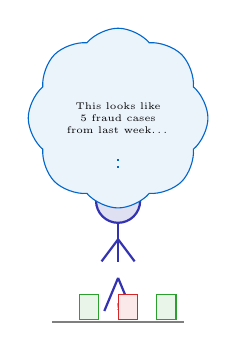
\begin{tikzpicture}[scale=0.7, every node/.style={transform shape}]
% Analyst at desk
\node[circle, draw=mlpurple, fill=mlpurple!15, minimum size=8mm, line width=0.8pt] (head) at (0,3.5) {};
\node[font=\tiny] at (0,3.5) {?};
\draw[mlpurple, line width=0.8pt] (head.south) -- ++(0,-0.7);
\draw[mlpurple, line width=0.8pt] (-0.3,2.4) -- (0,2.8) -- (0.3,2.4);
\draw[mlpurple, line width=0.8pt] (0,2.1) -- (-0.25,1.5);
\draw[mlpurple, line width=0.8pt] (0,2.1) -- (0.25,1.5);
% Desk
\draw[mlgray, line width=1pt] (-1.2,1.3) -- (1.2,1.3);
% Papers on desk
\foreach \x/\c in {-0.7/mlgreen,0/mlred,0.7/mlgreen} {
  \draw[\c, fill=\c!10, line width=0.4pt] (\x,1.35) rectangle ++(0.35,0.45);
}
\node[font=\tiny,mlred] at (0,1.57) {!};
% Thought bubble
\node[cloud, draw=mlblue, fill=mlblue!8, cloud puffs=8, cloud puff arc=100,
      minimum width=2.5cm, minimum height=1.2cm, font=\tiny, align=center] at (0,5)
      {This looks like\\5 fraud cases\\from last week\ldots};
\draw[mlblue, dotted, line width=0.5pt] (0,4.1) -- (0,4.3);
\end{tikzpicture}
\end{columns}
\bottomnote{KNN: find the most similar past cases and let them vote on the new one}
\end{frame}

%% SLIDE 3: Learning Objectives
\begin{frame}[t]{What Will You Learn in This Lecture?}
\small
\textbf{Learning Objectives}
\begin{enumerate}
\item \footnotesize \highlight{Derive} the distance-based classification rule and analyze its error bounds
\item \footnotesize \highlight{Evaluate} how $K$ controls the bias--variance tradeoff in practice
\item \footnotesize \highlight{Analyze} why feature scaling and dimensionality affect KNN performance
\item \footnotesize \highlight{Apply} cross-validation to select optimal $K$ for financial datasets
\end{enumerate}

\vspace{4mm}
\begin{columns}[T]
\column{0.48\textwidth}
\begin{block}{Prerequisites}
\footnotesize Basic probability, linear/logistic regression concepts (L01--L02).
\end{block}

\column{0.48\textwidth}
\begin{block}{Why It Matters}
\footnotesize KNN is the foundation of all distance-based methods and instance-based reasoning.
\end{block}
\end{columns}
\bottomnote{Bloom's levels: derive (4), evaluate (5), analyze (4), apply (3)}
\end{frame}

%% SLIDE 4: Plain English Definition
\begin{frame}[t]{What Is KNN in Plain English?}
\begin{columns}[T]
\column{0.50\textwidth}
\small
\textbf{The simplest classifier imaginable}

\footnotesize
Find the $K$ training points closest to the query. Let them vote. Majority wins.
\begin{compactlist}
\item \footnotesize No training phase --- just store the data
\item \footnotesize Non-parametric: no assumed functional form
\item \footnotesize Each prediction has an intuitive explanation
\end{compactlist}

\vspace{2mm}
\highlight{Analogy:} ``Asking your 5 nearest neighbors which restaurant to go to.''

\column{0.48\textwidth}
\vspace{2mm}
\footnotesize
\textbf{Key Vocabulary}
\begin{compactlist}
\item \footnotesize \textbf{Query point:} the new observation to classify
\item \footnotesize \textbf{Neighbor:} a training point close to the query
\item \footnotesize \textbf{Distance:} how we measure ``close''
\item \footnotesize \textbf{Majority vote:} most common label among $K$ neighbors
\item \footnotesize \textbf{$K$:} the number of neighbors to consult
\end{compactlist}
\end{columns}
\bottomnote{No formulas needed yet --- KNN is purely intuitive at this stage}
\end{frame}

%% SLIDE 5: Parametric vs Non-Parametric
\begin{frame}[t]{Where Does KNN Fit in Machine Learning?}
\begin{columns}[T]
\column{0.48\textwidth}
\small
\textbf{Parametric Models}

\footnotesize
\begin{compactlist}
\item \footnotesize Learn fixed coefficients (e.g., logistic regression)
\item \footnotesize Fast prediction --- just plug in
\item \footnotesize Model complexity is fixed after training
\end{compactlist}

\vspace{2mm}
\textcolor{mlblue}{Example:} $\hat{y} = \sigma(\beta_0 + \beta_1 x_1 + \beta_2 x_2)$

\column{0.48\textwidth}
\small
\textbf{Non-Parametric Models}

\footnotesize
\begin{compactlist}
\item \footnotesize Store all training data (e.g., KNN)
\item \footnotesize Flexible decision boundaries
\item \footnotesize Complexity grows with data size
\end{compactlist}

\vspace{2mm}
\textcolor{mlblue}{Example:} Find $K$ nearest, vote on class
\end{columns}

\vspace{3mm}
\begin{block}{Bridge}
\footnotesize KNN is the simplest non-parametric classifier. Understanding it builds intuition for all distance-based methods.
\end{block}
\bottomnote{Parametric = learn parameters. Non-parametric = memorize data.}
\end{frame}

%% ================================================================
%% CORE ZONE --- METHOD (Slides 6--14)
%% ================================================================

%% SLIDE 6: KNN Step-by-Step (Chart + text)
\begin{frame}[t]{How Does KNN Classify a New Point?}
\begin{columns}[T]
\column{0.55\textwidth}
\begin{center}

\includegraphics[width=\textwidth]{09_knn_step_by_step/chart}
\end{center}

\column{0.43\textwidth}
\small
\textbf{The Algorithm}

\footnotesize
\begin{enumerate}
\item \footnotesize Compute distance from query to \highlight{all} training points
\item \footnotesize Sort by distance (ascending)
\item \footnotesize Take the $K$ nearest neighbors
\item \footnotesize Count class votes $\to$ assign majority class
\end{enumerate}

\vspace{2mm}
\begin{block}{Key Insight}
\footnotesize No ``learning'' happens --- prediction = a lookup + a vote.
\end{block}
\end{columns}
\bottomnote{KNN is a \emph{lazy learner}: all computation happens at prediction time}
\end{frame}

%% SLIDE 7: Decision Boundaries (Full-size chart)
\begin{frame}[t]{What Do Different Decision Boundaries Look Like?}
\begin{center}

\includegraphics[width=0.65\textwidth]{01_knn_boundaries/chart}
\end{center}

\vspace{2mm}
\footnotesize
\textcolor{mlblue}{$K{=}1$: jagged, overfits noise.}
\quad \textcolor{mlorange}{$K{=}15$: smooth, may underfit.}
\quad \textcolor{mlgreen}{$K{=}5$: balanced tradeoff.}
\bottomnote{Decision boundaries become smoother as $K$ increases}
\end{frame}

%% SLIDE 8: Distance Metrics (Chart + formulas)
\begin{frame}[t]{How Do We Measure Distance?}
\begin{columns}[T]
\column{0.52\textwidth}
\begin{center}

\includegraphics[width=\textwidth]{02_distance_metrics/chart}
\end{center}

\column{0.46\textwidth}
\small
\textbf{Three Distance Functions}

\vspace{2mm}
\footnotesize
\textcolor{mlblue}{\textbf{Euclidean} (straight line):}
\[d_2(\mathbf{x}, \mathbf{y}) = \sqrt{\sum_{i=1}^{p}(x_i - y_i)^2}\]

\textcolor{mlorange}{\textbf{Manhattan} (city blocks):}
\[d_1(\mathbf{x}, \mathbf{y}) = \sum_{i=1}^{p}|x_i - y_i|\]

\textcolor{mlpurple}{\textbf{Minkowski} (generalized):}
\[d_q(\mathbf{x}, \mathbf{y}) = \left(\sum_{i=1}^{p}|x_i - y_i|^q\right)^{1/q}\]
\end{columns}
\bottomnote{Euclidean ($q{=}2$) and Manhattan ($q{=}1$) are special cases of Minkowski}
\end{frame}

%% SLIDE 9: Worked Example (Table + calculation)
\begin{frame}[t]{Worked Example: Which Transaction Is the Nearest Neighbor?}
\small
\textbf{Training data} (4 past transactions):

\vspace{1mm}
\footnotesize
\begin{tabular}{ccccc}
\toprule
\textbf{ID} & \textbf{Amount (\$)} & \textbf{Time (hr)} & \textbf{Foreign} & \textbf{Label} \\
\midrule
\#1 & 500 & 13 & 1 & Fraud \\
\#2 & 420 & 15 & 1 & Fraud \\
\#3 & 200 & 10 & 0 & Legit \\
\#4 & 480 & 12 & 1 & Legit \\
\bottomrule
\end{tabular}

\vspace{2mm}
\textbf{Query:} Amount=450, Time=14, Foreign=1 \quad (Euclidean distance)

\vspace{1mm}
\footnotesize
\begin{tabular}{cl}
\toprule
\textbf{ID} & \textbf{Distance} \\
\midrule
\#1 & $\sqrt{(450{-}500)^2 + (14{-}13)^2 + (1{-}1)^2} = \sqrt{2501} \approx 50.0$ \\
\#2 & $\sqrt{(450{-}420)^2 + (14{-}15)^2 + (1{-}1)^2} = \sqrt{901} \approx 30.0$ \\
\#3 & $\sqrt{(450{-}200)^2 + (14{-}10)^2 + (1{-}0)^2} = \sqrt{62517} \approx 250.0$ \\
\#4 & $\sqrt{(450{-}480)^2 + (14{-}12)^2 + (1{-}1)^2} = \sqrt{904} \approx 30.1$ \\
\bottomrule
\end{tabular}

\vspace{2mm}
\highlight{$K{=}3$}: Neighbors \#2, \#4, \#1 $\to$ 2 Fraud, 1 Legit $\to$ \textcolor{mlred}{\textbf{Predict FRAUD}}
\bottomnote{Note: Amount dominates the distance --- we will fix this with feature scaling (Slide 12)}
\end{frame}

%% SLIDE 10: Formal Decision Rule (Definition block)
\begin{frame}[t]{The KNN Decision Rule Formally}
\begin{block}{KNN Classifier}
\[
\hat{y}(\mathbf{x}) = \arg\max_{c \in \mathcal{C}} \sum_{i \in N_K(\mathbf{x})} \mathbb{1}(y_i = c)
\]
where $N_K(\mathbf{x})$ = set of $K$ nearest neighbors of $\mathbf{x}$.
\end{block}

\vspace{3mm}
\begin{block}{Probability Estimate}
\[
\hat{P}(Y{=}c \mid \mathbf{x}) = \frac{1}{K}\sum_{i \in N_K(\mathbf{x})} \mathbb{1}(y_i = c)
\]
\end{block}

\vspace{3mm}
\footnotesize
\highlight{Translation:} Count the votes among the $K$ nearest neighbors. The class with the most votes wins.

\vspace{2mm}
\textbf{Example from Slide 9:} $\hat{P}(\text{Fraud} \mid \mathbf{x}_q) = \frac{2}{3} = 0.67$, \quad $\hat{P}(\text{Legit} \mid \mathbf{x}_q) = \frac{1}{3} = 0.33$
\bottomnote{The indicator function $\mathbb{1}(\cdot)$ returns 1 if true, 0 otherwise}
\end{frame}

%% SLIDE 11: Bias-Variance Tradeoff (Chart + text)
\begin{frame}[t]{How Does $K$ Control Bias and Variance?}
\begin{columns}[T]
\column{0.55\textwidth}
\begin{center}

\includegraphics[width=\textwidth]{10_bias_variance_visual/chart}
\end{center}

\column{0.43\textwidth}
\small
\textbf{The Tradeoff}

\vspace{2mm}
\footnotesize
\textcolor{mlred}{\textbf{Small $K$ (e.g., 1):}}
\begin{compactlist}
\item \footnotesize Low bias, \highlight{high variance}
\item \footnotesize Complex, noisy boundaries
\end{compactlist}

\vspace{2mm}
\textcolor{mlblue}{\textbf{Large $K$ (e.g., 50):}}
\begin{compactlist}
\item \footnotesize \highlight{High bias}, low variance
\item \footnotesize Smooth, potentially wrong boundaries
\end{compactlist}

\vspace{2mm}
\begin{block}{Goal}
\footnotesize Find the $K$ that minimizes \highlight{test error}.
\end{block}
\end{columns}
\bottomnote{This is the fundamental tradeoff in all of machine learning --- not just KNN}
\end{frame}

%% SLIDE 12: Feature Scaling (Chart + text)
\begin{frame}[t]{Why Must We Scale Features?}
\begin{columns}[T]
\column{0.55\textwidth}
\begin{center}

\includegraphics[width=\textwidth]{08_feature_scaling_effect/chart}
\end{center}

\column{0.43\textwidth}
\small
\textbf{The Problem}

\footnotesize
If Amount $\in [0, 10000]$ and Time $\in [0, 24]$, distance is \highlight{dominated by Amount}.

\vspace{3mm}
\textbf{The Solution}

\footnotesize
\textcolor{mlblue}{StandardScaler}: transform each feature to mean$=0$, std$=1$:
\[z_i = \frac{x_i - \bar{x}_i}{\sigma_i}\]

\vspace{2mm}
\begin{block}{Rule}
\footnotesize \highlight{Always} scale features \emph{before} computing distances.
\end{block}
\end{columns}
\bottomnote{Fit the scaler on training data only --- transform test data with the same parameters}
\end{frame}

%% SLIDE 13: Curse of Dimensionality (Two-column text)
\begin{frame}[t]{The Curse of Dimensionality}
\begin{columns}[T]
\column{0.48\textwidth}
\small
\textbf{The Problem}

\footnotesize
In high dimensions, \highlight{all points become roughly equidistant}.
\begin{compactlist}
\item \footnotesize Volume of unit hypersphere $\to 0$ as $d \to \infty$
\item \footnotesize Data needed grows exponentially: $n \propto k^d$
\item \footnotesize Nearest neighbor is barely closer than the farthest
\end{compactlist}

\column{0.48\textwidth}
\small
\textbf{Practical Guidance}

\footnotesize
KNN works well when $p < 20$ features.
\begin{compactlist}
\item \footnotesize \textbf{Mitigation 1:} PCA to reduce dimensions ($\to$ L05)
\item \footnotesize \textbf{Mitigation 2:} Feature selection (keep only informative features)
\item \footnotesize \textbf{Mitigation 3:} Use approximate nearest neighbors (e.g., Annoy, FAISS)
\end{compactlist}
\end{columns}

\vspace{3mm}
\begin{block}{Key Insight}
\footnotesize Distance loses meaning in high dimensions --- ``closeness'' stops discriminating.
\end{block}
\bottomnote{This curse affects ALL distance-based methods, not just KNN}
\end{frame}

%% SLIDE 14: Cover-Hart Error Bound (Theorem block)
\begin{frame}[t]{Error Bound: How Good Can KNN Be?}
\begin{block}{Cover \& Hart Theorem (1967)}
As $n \to \infty$, the 1-NN error rate $R_{1\text{-NN}}$ satisfies:
\[
R^* \;\leq\; R_{1\text{-NN}} \;\leq\; 2\,R^*\!\left(1 - R^*\right)
\]
where $R^*$ is the Bayes optimal error rate.
\end{block}

\vspace{3mm}
\footnotesize
\textbf{What does this mean?}
\begin{compactlist}
\item \footnotesize 1-NN error is at most \highlight{twice} the theoretical minimum
\item \footnotesize If Bayes error is 5\%: $R_{1\text{-NN}} \leq 2 \times 0.05 \times 0.95 = 9.5\%$
\item \footnotesize Remarkable guarantee for such a simple algorithm
\end{compactlist}

\vspace{2mm}
\begin{block}{Caveat}
\footnotesize Requires $n \to \infty$ and fixed dimensionality. In practice, performance depends on $K$, scaling, and $p$.
\end{block}
\bottomnote{Cover \& Hart (1967), ``Nearest neighbor pattern classification,'' IEEE Trans.\ Info.\ Theory}
\end{frame}

%% ================================================================
%% CORE ZONE --- SOLUTION (Slides 15--19)
%% ================================================================

%% SLIDE 15: Cross-Validation for K (Chart + method)
\begin{frame}[t]{How Do We Select the Best $K$?}
\begin{columns}[T]
\column{0.55\textwidth}
\begin{center}

\includegraphics[width=\textwidth]{13_cv_accuracy_curve/chart}
\end{center}

\column{0.43\textwidth}
\small
\textbf{5-Fold Cross-Validation}

\footnotesize
\begin{enumerate}
\item \footnotesize For $K = 1, 3, 5, \ldots, 21$
\item \footnotesize Split training data into 5 folds
\item \footnotesize Train on 4 folds, test on 1
\item \footnotesize Average accuracy across folds
\item \footnotesize Pick $K$ with highest mean CV accuracy
\end{enumerate}

\vspace{2mm}
\begin{block}{Practical Tips}
\footnotesize Use \highlight{odd} $K$ for binary tasks (avoids ties). Try $K \in [1, \sqrt{n}]$.
\end{block}
\end{columns}
\bottomnote{Cross-validation prevents overfitting to the training set when tuning $K$}
\end{frame}

%% SLIDE 16: Weighted KNN (Two-column)
\begin{frame}[t]{Weighted KNN: Not All Neighbors Are Equal}
\begin{columns}[T]
\column{0.48\textwidth}
\small
\textbf{Standard KNN}

\footnotesize
All $K$ neighbors vote equally:
\begin{compactlist}
\item \footnotesize Neighbor at distance 1 counts the same as neighbor at distance 10
\item \footnotesize Sensitive to outliers among the $K$ neighbors
\end{compactlist}

\column{0.48\textwidth}
\small
\textbf{Weighted KNN}

\footnotesize
Closer neighbors get more weight:
\[w_i = \frac{1}{d(\mathbf{x}, \mathbf{x}_i)^2}\]
\begin{compactlist}
\item \footnotesize Nearby neighbors dominate the vote
\item \footnotesize Less sensitive to large $K$
\end{compactlist}
\end{columns}

\vspace{3mm}
\footnotesize
\textbf{Worked example:} 3 neighbors at distances $d{=}1, 3, 5$

\vspace{1mm}
\begin{tabular}{cccc}
\toprule
\textbf{Distance} & \textbf{Weight} $1/d^2$ & \textbf{Label} & \textbf{Weighted Vote} \\
\midrule
1.0 & 1.000 & Fraud & 1.000 \\
3.0 & 0.111 & Legit & 0.111 \\
5.0 & 0.040 & Legit & 0.040 \\
\bottomrule
\end{tabular}
\quad Fraud: 1.00 vs.\ Legit: 0.15 $\to$ \textcolor{mlred}{\textbf{Predict FRAUD}}
\bottomnote{In sklearn: \texttt{KNeighborsClassifier(weights='distance')}}
\end{frame}

%% SLIDE 17: Interpreting KNN Predictions (Step-by-step)
\begin{frame}[t]{Interpreting KNN Predictions}
\small
\textbf{Why KNN is inherently interpretable}

\vspace{2mm}
\footnotesize
For a fraud detection prediction with $K{=}5$:

\vspace{2mm}
\begin{tabular}{cccccc}
\toprule
\textbf{Neighbor} & \textbf{Amount} & \textbf{Time} & \textbf{Foreign} & \textbf{Distance} & \textbf{Label} \\
\midrule
\#1 & \$480 & 14:30 & Yes & 0.12 & \textcolor{mlred}{Fraud} \\
\#2 & \$460 & 13:50 & Yes & 0.18 & \textcolor{mlred}{Fraud} \\
\#3 & \$445 & 14:10 & Yes & 0.21 & \textcolor{mlred}{Fraud} \\
\#4 & \$470 & 15:00 & No  & 0.35 & \textcolor{mlgreen}{Legit} \\
\#5 & \$500 & 13:00 & Yes & 0.40 & \textcolor{mlgreen}{Legit} \\
\bottomrule
\end{tabular}

\vspace{3mm}
$\hat{P}(\text{Fraud}) = 3/5 = 0.60$ \quad $\to$ \textcolor{mlred}{\textbf{Flagged as Fraud}}

\vspace{3mm}
\begin{block}{Explanation Template}
\footnotesize ``This transaction was flagged because 3 of its 5 most similar past transactions were confirmed fraud --- all had similar amount, time, and foreign status.''
\end{block}
\bottomnote{KNN gives case-based explanations: show the evidence, not abstract coefficients}
\end{frame}

%% SLIDE 18: KNN for Regression (Definition + example)
\begin{frame}[t]{KNN for Regression}
\begin{block}{KNN Regression Rule}
\[
\hat{y}(\mathbf{x}) = \frac{1}{K}\sum_{i \in N_K(\mathbf{x})} y_i
\]
Predict the \highlight{average} of the $K$ nearest neighbors' target values.
\end{block}

\vspace{3mm}
\footnotesize
\textbf{Worked example:} Predict house price from 3 nearest neighbors

\vspace{1mm}
\begin{tabular}{cccc}
\toprule
\textbf{Neighbor} & \textbf{Size (sqm)} & \textbf{Distance} & \textbf{Price (k\euro{})} \\
\midrule
\#1 & 82 & 0.15 & 320 \\
\#2 & 78 & 0.22 & 290 \\
\#3 & 85 & 0.31 & 345 \\
\bottomrule
\end{tabular}

\vspace{2mm}
$\hat{y} = \frac{320 + 290 + 345}{3} = \text{318.3k\euro{}}$

\vspace{2mm}
Weighted: $\hat{y}_w = \frac{320/0.15^2 + 290/0.22^2 + 345/0.31^2}{1/0.15^2 + 1/0.22^2 + 1/0.31^2} \approx 314.5$k\euro{}
\bottomnote{In sklearn: \texttt{KNeighborsRegressor(n\_neighbors=3, weights='distance')}}
\end{frame}

%% SLIDE 19: Computational Complexity (Two-column)
\begin{frame}[t]{Computational Complexity: The Speed Problem}
\begin{columns}[T]
\column{0.48\textwidth}
\small
\textbf{Brute Force}

\footnotesize
$O(n \times p)$ per query --- must scan ALL training points.
\begin{compactlist}
\item \footnotesize 1M training, 100 features = 100M operations per prediction
\item \footnotesize \highlight{Training}: $O(1)$ --- just store the data
\item \footnotesize \highlight{Prediction}: $O(n \times p)$ --- expensive!
\end{compactlist}

\column{0.48\textwidth}
\small
\textbf{Acceleration Structures}

\footnotesize
\begin{compactlist}
\item \footnotesize \textbf{KD-Trees}: $O(p \log n)$ per query (low $p$)
\item \footnotesize \textbf{Ball Trees}: $O(p \log n)$ per query (any metric)
\item \footnotesize \textbf{Approximate NN}: sub-linear (FAISS, Annoy)
\end{compactlist}

\vspace{2mm}
\begin{block}{sklearn}
\footnotesize \texttt{algorithm='auto'} picks the best structure for your data.
\end{block}
\end{columns}

\vspace{3mm}
\footnotesize
\highlight{Bottom line:} KNN prediction is \emph{slow} compared to parametric models. This limits real-time applications.
\bottomnote{KNN trades training speed for prediction speed --- opposite of neural networks}
\end{frame}

%% ================================================================
%% CLOSING ZONE (Slides 20--25)
%% ================================================================

%% SLIDE 20: Pros and Cons
\begin{frame}[t]{When to Use KNN --- and When Not To}
\begin{columns}[T]
\column{0.48\textwidth}
\small
\textcolor{mlgreen}{\textbf{Strengths}}

\footnotesize
\begin{compactlist}
\item \footnotesize \textcolor{mlgreen}{\checkmark} No training phase needed
\item \footnotesize \textcolor{mlgreen}{\checkmark} Handles multi-class naturally
\item \footnotesize \textcolor{mlgreen}{\checkmark} Non-linear decision boundaries
\item \footnotesize \textcolor{mlgreen}{\checkmark} Intuitive case-based explanations
\item \footnotesize \textcolor{mlgreen}{\checkmark} Simple to implement and tune
\end{compactlist}

\column{0.48\textwidth}
\small
\textcolor{mlred}{\textbf{Limitations}}

\footnotesize
\begin{compactlist}
\item \footnotesize \textcolor{mlred}{$\times$} Slow prediction ($O(np)$)
\item \footnotesize \textcolor{mlred}{$\times$} Curse of dimensionality ($p > 20$)
\item \footnotesize \textcolor{mlred}{$\times$} Requires feature scaling
\item \footnotesize \textcolor{mlred}{$\times$} Stores entire training set in memory
\item \footnotesize \textcolor{mlred}{$\times$} Sensitive to irrelevant features
\end{compactlist}
\end{columns}

\vspace{3mm}
\begin{block}{Rule of Thumb}
\footnotesize Use KNN when: few features ($p < 20$), moderate $n$, need interpretability. Avoid when: large $n$, high $p$, real-time prediction required.
\end{block}
\bottomnote{KNN is an excellent baseline --- always try it before complex models}
\end{frame}

%% SLIDE 21: KNN vs Logistic Regression (Comparison table)
\begin{frame}[t]{KNN vs Logistic Regression for Fraud Detection}
\small
\vspace{1mm}
\footnotesize
\begin{tabular}{lll}
\toprule
\textbf{Criterion} & \textbf{KNN} & \textbf{Logistic Regression} \\
\midrule
Interpretability & Case-based (show neighbors) & Coefficient-based (log-odds) \\
Non-linearity & Yes (inherently) & No (needs feature engineering) \\
Training speed & $O(1)$ --- just store & $O(np)$ --- optimization \\
Prediction speed & $O(np)$ --- \textcolor{mlred}{slow} & $O(p)$ --- \textcolor{mlgreen}{fast} \\
Feature scaling & \highlight{Required} & Not required \\
High dimensions & Degrades ($p > 20$) & Handles well (with regularization) \\
Real-time use & Limited & \textcolor{mlgreen}{Excellent} \\
\bottomrule
\end{tabular}

\vspace{3mm}
\begin{block}{When to Choose Which?}
\footnotesize \textbf{KNN:} Few features, need case-based audit trail, non-linear patterns. \quad \textbf{LR:} Many features, real-time scoring, regulatory transparency.
\end{block}
\bottomnote{In banking: logistic regression for real-time scoring, KNN for post-hoc investigation}
\end{frame}

%% SLIDE 22: Code Example (fragile frame)
\begin{frame}[fragile,t]{Hands-On: Build a Fraud Detector with KNN}
\small
\textbf{Complete sklearn workflow}

\vspace{2mm}
\footnotesize
\begin{semiverbatim}
\textcolor{mlgray}{# Step 1: Scale features}
\textcolor{mlblue}{from} sklearn.neighbors \textcolor{mlblue}{import} KNeighborsClassifier
\textcolor{mlblue}{from} sklearn.preprocessing \textcolor{mlblue}{import} StandardScaler
\textcolor{mlblue}{from} sklearn.model_selection \textcolor{mlblue}{import} cross_val_score

scaler = StandardScaler()
X_train_s = scaler.fit_transform(X_train)
X_test_s  = scaler.transform(X_test)

\textcolor{mlgray}{# Step 2: Fit and evaluate}
knn = KNeighborsClassifier(n_neighbors=5, weights=\textcolor{mlorange}{'distance'})
scores = cross_val_score(knn, X_train_s, y_train, cv=5)
print(f\textcolor{mlorange}{"CV Accuracy: \{scores.mean():.3f\} +/- \{scores.std():.3f\}"})

\textcolor{mlgray}{# Step 3: Final prediction}
knn.fit(X_train_s, y_train)
y_pred = knn.predict(X_test_s)
\end{semiverbatim}

\vspace{2mm}
\footnotesize
Full notebook: \texttt{L03\_knn.ipynb} on Colab
\bottomnote{Remember: fit scaler on training data only, then transform both train and test}
\end{frame}

%% SLIDE 23: Key Takeaways (Two-column summary)
\begin{frame}[t]{Key Takeaways}
\begin{columns}[T]
\column{0.48\textwidth}
\small
\textcolor{mlpurple}{\textbf{Concepts}}

\footnotesize
\begin{compactlist}
\item \footnotesize Distance metrics (Euclidean, Manhattan, Minkowski)
\item \footnotesize Majority vote classification rule
\item \footnotesize Bias--variance tradeoff via $K$
\item \footnotesize Curse of dimensionality
\item \footnotesize Cover--Hart error bound
\end{compactlist}

\column{0.48\textwidth}
\small
\textcolor{mlpurple}{\textbf{Practice}}

\footnotesize
\begin{compactlist}
\item \footnotesize \highlight{Always} scale features before KNN
\item \footnotesize Use cross-validation to select $K$
\item \footnotesize Consider weighted KNN for noisy data
\item \footnotesize Watch out for high dimensions ($p > 20$)
\item \footnotesize Use KD-Trees / Ball Trees for large $n$
\end{compactlist}
\end{columns}

\vspace{4mm}
\begin{block}{One Sentence Summary}
\footnotesize KNN classifies by finding the most similar past observations and letting them vote --- simple, powerful, and inherently interpretable.
\end{block}
\bottomnote{KNN is the starting point for understanding all distance-based and instance-based methods}
\end{frame}

%% SLIDE 24: Bridge to K-Means
\begin{frame}[t]{What's Next: Unsupervised Learning with K-Means}
\small
\textbf{From labeled to unlabeled data}

\vspace{3mm}
\footnotesize
\begin{columns}[T]
\column{0.48\textwidth}
\textbf{What we just learned (KNN):}
\begin{compactlist}
\item \footnotesize Uses \highlight{labels} to classify
\item \footnotesize Supervised: given correct answers
\item \footnotesize Goal: predict the label of new points
\end{compactlist}

\column{0.48\textwidth}
\textbf{What's coming (K-Means):}
\begin{compactlist}
\item \footnotesize Has \highlight{no labels} at all
\item \footnotesize Unsupervised: discover structure
\item \footnotesize Goal: find natural groups in data
\end{compactlist}
\end{columns}

\vspace{4mm}
\begin{block}{Teaser}
\footnotesize Same distance idea, completely different goal: K-Means finds customer segments without predefined groups. Can a bank discover its own customer types?
\end{block}
\bottomnote{Next lecture: K-Means Clustering --- from distance-based classification to distance-based grouping}
\end{frame}

%% SLIDE 25: XKCD Closing
\begin{frame}[t]{Closing Thought}
\begin{center}
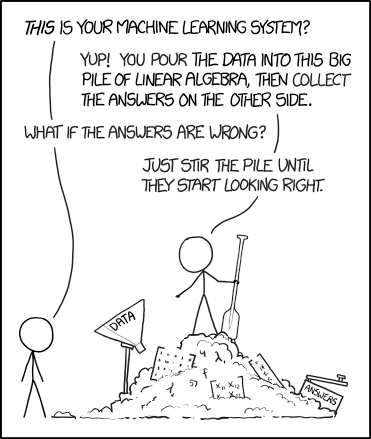
\includegraphics[height=0.55\textheight]{images/1838_machine_learning.png}
\end{center}
\vspace{-1mm}
\footnotesize
\begin{center}
\emph{``Sometimes the simplest ideas work best --- ask the 5 nearest transactions.''}
\end{center}
\bottomnote{XKCD \#1838 by Randall Munroe (CC BY-NC 2.5)}
\end{frame}

\end{document}
